\section{Configuration energy}
\label{section:configuration_energy}
The configuration energy is the energy consumed when transferring a model from the off-chip memory to the GrAICore's on-chip memories.

\subsection{Configuration process}
We explore the potential of integrating the DDR (double data rate) interface as a future external memory solution for the \graicore{}.
The integration of a DDR interface could bring about substantial benefits in performance.
Its high bandwidth has the potential to rapidly transfer AI models between the off-chip and on-chip memory, leading to faster configuration times.
Moreover, DDR memory, such as LPDDR5X \cite{JEDEC_JESD209-5C}, is designed with energy efficiency in mind, which contributes to low-power operations.
This type of DRAM offers high density, providing the possibility for accommodating more and larger AI models on a smaller silicon area.
This makes DDR a promising solution for model (re)configuration on the \graicore{}.

Furthermore, we also investigate the potential of using PCM in conjunction with the DDR interface.
PCM's non-volatility and high-speed operation, combined with the high bandwidth of DDR, could significantly improve the overall performance of the system.

\begin{figure}[hbtp]
    \centering
    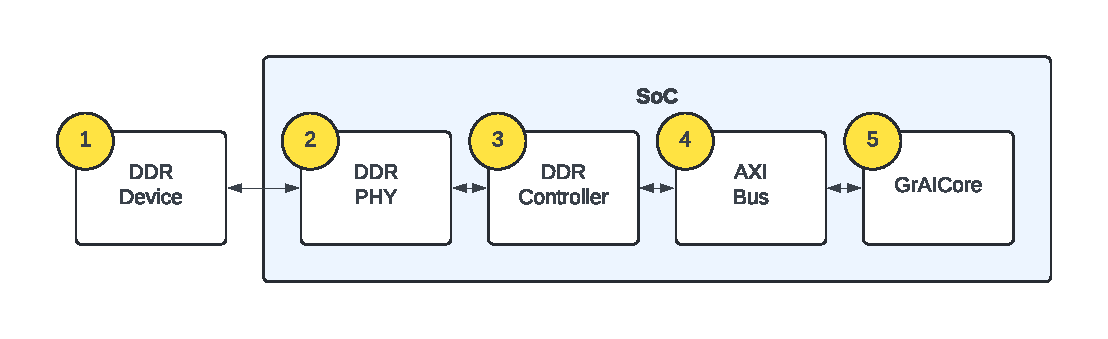
\includegraphics[width=\linewidth]{assets/ddr_graicore_block_diagram.pdf}
    \caption{
        Interconnection of the external memory device and \graicore{}
    }
    \label{fig:ddr_graicore_block_diagram}
\end{figure}

A typical system with external memory and DDR interface looks as shown in \cref{fig:ddr_graicore_block_diagram}.
\begin{description}
    \item[Memory device:] 
    The physical component where (model) data is stored and read from.
    This typically takes the form of an integrated circuit that contains an array of memory cells.
    These cells hold individual bits of information, and they are organized into a structured format to allow for efficient access.
    \item[DDR PHY:] 
    A crucial component that bridges the gap between the \graicore{}'s digital signals and the analog signals required by the memory device.
    It manages the high-speed signaling, precise timing, and voltage levels necessary for reliable communication.
    The DDR PHY serializes data from the DDR controller for transmission and deserializes incoming data, ensuring proper data transfer.
    \item[DDR Controller:] 
    This component is responsible for managing all memory operations.
    It acts as an intermediary between the \graicore{} and the memory device, translating the requests from the \graicore{}, such as read and write requests, into the specific control signals required by the memory device.
    The DDR controller also manages essential functions like memory refresh, power management and error correction.
    \item[AXI Bus:] 
    The AXI bus (Advanced eXtensible Interface) is a standardized, high-performance interconnect used to connect different components within a SoC \cite{ARM_AXI_Specification}.
    It enables parallel data transfer, facilitating high bandwidth and low latency communication between the components.
    \item[\graicore{}:] 
    The major components of the \graicore{} that contribute to the configuration energy is the data transfers through its \confignoc{} and the writing of data to the SRAMs.
\end{description}

The model reconfiguration process is initiated by an external host, typically a microcontroller.
The host transmits a command to the DDR controller serving as the explicit trigger to initiate the data transfer process.
Upon receiving this command, the DDR controller, responsible for managing the external memory, initiates the necessary sequence of operations.
The DDR PHY then transmits the read command to the external memory.
Once the data is retrieved, it is transmitted back to the DDR controller via the DDR PHY.

The DDR controller then encapsulates this raw data into AXI transactions.
These AXI transactions, carrying the data payload, are then transmitted over the AXI bus.
This bus acts as a primary interconnect, facilitating high-bandwidth data movement between different modules within the \graicore{}.
The AXI transactions traverse the AXI bus until they reach the entry point of the \confignoc{}.

At the \confignoc{}'s entry point, the data undergoes a transformation into a packetized format, as detailed in \cref{section:improved_packet_format}.
This packetization process prepares the data for efficient transmission across the \confignoc{}, which employs packet-switching mechanisms for data routing and delivery.
The \confignoc{}'s routing logic analyzes the packet headers and determines the path to the designated destination within the \graicore{}.
The packets traverse the \confignoc{}, potentially hopping between multiple routers and links, until they arrive at the target neuron core.
The data is then written into specific memory locations within the neuron core's SRAM, determined by a predefined mapping scheme or address translation mechanism.
With the data now residing in the neuron core's SRAM, it becomes readily available for processing by the neuron core.

\subsection{Modeling}
For the analysis, we assume that we are using the newly proposed \confignoc{} in \cref{sec:proposed_noc}. 
With the new packet format, a packet contains at most 64 data phits of 64 bits each.
That is, a maximum of 512 bytes\footnote{$64 \times \frac{\SI{64}{b}}{8} = \SI{512}{B}$} of payload per packet.
Furthermore, an additional injection point is introduced (see \cref{fig:segmentation_example_2}).
Next to the injection point connected to the router on the bottom left of the \confignoc{}, a new one is added and connected to the router six positions up.

To estimate the energy cost for configuration, we require the following information from a model:
\begin{itemize}
    \item Amount of data to transfer to the SRAMs
    \item Destination neuron core of the data
\end{itemize}

The amount of data to transfer determines how much data will be read, transferred and written.
We are assuming that the same amount of data read from the external memory is written to the SRAMs.
The location (specific neuron core) of the data determines the number of hops the data has to perform in the \confignoc{}.
The amount of data to write can also be used to determine the configuration time.
The configuration time is calculated by dividing the amount of data with the write bandwidth.

The amount of data to be written and to which neuron cores depends on how the compiler has performed the mapping on the \graicore{}.
Phits that need to be transferred to neuron cores further away from an injection point will require more hops to reach, and therefore consume more energy than neuron cores closer to an injection point.
Furthermore, the amount of data that needs to be written to each core differs.
We can retrieve this information from the compiler artifacts.

For estimating the energy for the \graicore{} component, we consider the \confignoc{} and the SRAMs.
These are the main components for the energy consumption in the \graicore{}.
The \confignoc{} consumes energy by transferring the phits to its destinations via one or multiple hops through the NoC.
The SRAM consumes energy by writing the data to its banks.

The configuration energy consists of the reading, transferring and writing of data from the external memory to the \graicore{}'s SRAMs. 
Let $C$ be the set of tuples holding the coordinates of every core:
\begin{equation*}
    C = \{\,\left(x,y\right) \in \mathbb{N}^2 \mid 0 \leq x \leq 11 \wedge 0 \leq y \leq 11 \,\} 
\end{equation*}

\Cref{fig:model_data_heapmap} shows for an $80\%$ pruned version of ResNet-50 the amount of data that needs to be written to each of the 144 neuron cores.
We observe that the data is not uniformly distributed across the SRAMs.
Therefore, we require information how much data needs to be transferred to each SRAM.

\begin{figure}[hbtp]
    \centering
    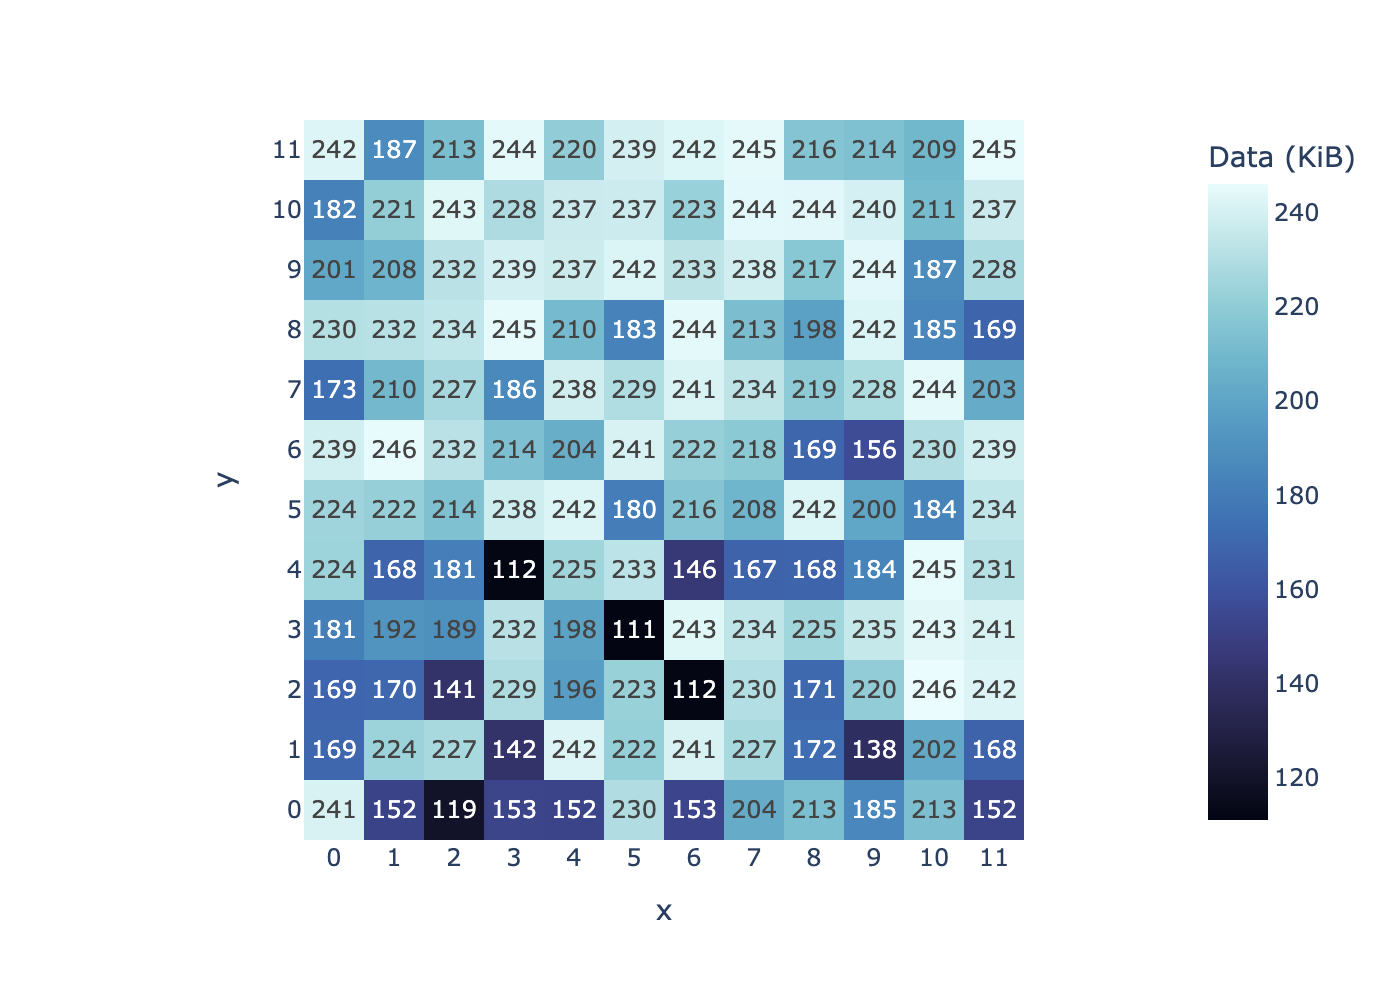
\includegraphics[clip, trim=80 20 10 30, width=0.8\linewidth]{assets/resnet50_coredata_heatmap.png}
    \caption{Amount of data to be written to each neuron core for the ResNet-50 model (80\% pruned).}
    \label{fig:model_data_heapmap}
\end{figure}

Let $D$ be a matrix of $12 \times 12$ with $D_{i,j}$ denoting the number of bytes to be written to core $\left( i,j \right)$.
This matrix can be constructed from the artifacts outputted by the compiler.

The number of phits to be transferred through the \confignoc{} influences the total energy costs.
In particular, the number of phits to be transferred affects the number of hops to be taken in total and the amount of data to be written to the SRAMs.
Therefore, we need to determine how many phits need to be transferred to each neuron core.
A packet can contain up to 64 data phits, that is $64 \times \SI{64}{b} = \SI{512}{B}$ of payload data.
Suppose we need to transfer $d$ bytes to a neuron core, we then require a total of $\left\lfloor \frac{d}{\SI{512}{B}} \right\rfloor$ packets with 64 data phits.
If $\left( d \bmod \SI{512}{B} \right) > 0$, then there is an additional packet for the remaining $\left( d \bmod \SI{512}{B} \right)$ bytes of data.
The remaining packet will consist of $\left\lceil \frac{d \bmod \SI{512}{B}}{\SI{8}{B}}\right\rceil$ data phits.
Note that each packet also contains a single phit of 64 bits for the header information.

The total energy cost for configuring the \graicore{} can be estimated with the following equation:
\begin{equation}
    \econf = \eread + \ephy + \ectrl + \eaxi + \enoc + \ewrite
\end{equation}
This equation sums up the energy consumption of all the major components that take part in the configuration process.

With:
\begin{align*} 
\eread &= 
    \sum_{c \in C}^{} D_c \times \ereadbyte \\
\ephy &=
    \sum_{c \in C}^{} D_c \times \ephybyte \\
\ectrl &=
    \sum_{c \in C}^{} D_c \times \ectrlbyte \\
\eaxi &=
    \sum_{c \in C}^{} D_c \times \eaxibyte \\
\enoc &=
    \ehopsixtyfourbits \times \sum_{c \in C}^{}{\nhops(c) \times \ptotal(D_c)} \\
\ewrite &=
    \ewritesixtyfourbits \times \sum_{c \in C}^{}{\pdata(D_c)}
\end{align*}

And:
\begin{align*} 
\nhops(x,y) &=
    \begin{cases} 
        x + y + 1 & \textrm{if } 0 \leq y \leq 5 \\
        x + y - 5 & \text{if } 6 \leq y \leq 11
    \end{cases}
    \\
    \pdata(d) &=
        \left\lfloor \frac{d}{\SI{512}{B}} \right\rfloor \times 64 + \left\lceil \frac{d \bmod \SI{512}{B}}{\SI{8}{B}} \right\rceil = \left\lceil \frac{d}{\SI{8}{B}} \right\rceil
    \\
    \pheader(d) &=
        \left\lfloor \frac{d}{\SI{512}{B}} \right\rfloor + 1
    \\
    \ptotal(d) &=
        \pdata(d) + \pheader(d)
\end{align*}

\begin{eqexpl}[30mm]
    \item{$\pdata(D_c)$} total data phits for transferring $D_c$ bytes
    \item{$\pheader(D_c)$} total header phits for transferring $D_c$ bytes
    \item{$\ptotal(D_c)$} total phits (includes headers) for transferring $D_c$ bytes
    \item{$\nhops(c)$} the number of hops required to reach the neuron core at coordinate $c$, starting from the router closest to the injection point. It has two sub-functions due to the new \confignoc{}'s dual injector architecture
    \item{$\ereadbyte$} energy for reading a single byte from the external memory device
    \item{$\ephybyte$} energy for transferring a single byte using the DDR PHY
    \item{$\ectrlbyte$} energy for transferring/processing a single byte by the DDR controller
    \item{$\eaxibyte$} energy for transferring a single byte using the AXI bus
    \item{$\ehopsixtyfourbits$} energy for performing a single hop of 64 bits in the \confignoc{}
    \item{$\ewritesixtyfourbits$} energy for writing back 64 bits to a neuron core's SRAM
\end{eqexpl}

